% !TEX root =  ../thesis.tex

%%%%%%%%%%%%%%%%%%%%%%%%%%%%%%%%%%%%%%%%%%
Once the lookup table has been constructed, it is then possible to proceed with an automated analysis of applications.
In this section we present the high level steps of the analysis, along with the challenges we face during this process, while the implementation details will be discussed in \autoref{chap:implem}.

\section{Privacy policy retrieval}
The first step is to retrieve the privacy policy, given an arbitrary application. This proved to be one significant challenge, for the following main reasons:
\begin{itemize}
    \item there is no legal requirement enforcing an Android application to have a privacy policy. Some applications simply do not provide one.
    \item there is no standard format for such documents. While the Play Store has a standard interface for providing a link to an app's privacy policy, the content of the link is arbitrary and completely at the discretion of the developer.
    \item some application developers do not provide a link to the privacy policy in the Play Store.
\end{itemize}

When present, the \emph{Privacy Policy} link in the Play Store interface can be followed to access the actual document, which can then be fetched in order to perform semantic analysis over it, as discussed in \autoref{sec:privacy-policy-analysis}.

For the purposes of this thesis, we limit our search for the privacy policy to the Play Store web interface. If the developer provided a privacy policy link, it is followed and analyzed, otherwise the search simply fails. This is a known limitation of this approach.

\section{Permissions retrieval}
The next step of the analysis involves retrieving the permissions list of an arbitrary Android application. This is a much easier task than retrieving the privacy policy, since every Android application is guaranteed to declare the requested permissions in a uniform format. The main challenge of this step is the implementation, due to the lack of official APIs to retrieve the desired information. Details of the solution are presented \autoref{chap:implem}.

\section{Privacy policy analysis}
\label{sec:privacy-policy-analysis}
Once the privacy policy document and the permissions list are both available, we can proceed with the semantic analysis.

First, the document is broken down into semantic sections, such as paragraphs and sentences.
Second, the keyword and expressions contained in the lookup table of each permission are matched against each section.
For each permission, the relevant matching sentences are then collected.

As discussed in \autoref{sec:false-positives}, we then identify false positive matches, i.e. the ones including verbs in the ``false positive table'', and exclude them from the final result set.

Such results are then presented to the final user, as discussed in the next section.

\section{User interface}
The results are made available to the user via a web interface. The interface allows the user to search for an arbitrary application on the Play Store; the permissions list and the privacy policy are then automatically retrieved, whenever possible.
The user has then the ability of selecting a specific permission, and a list of relevant sentences are extracted by the privacy policy and presented to them, along with an accurate description of the permission itself.

Such an interface allows the user to quickly evaluate the privacy-related risks of an Android application, by highlighting the relevant sections of the privacy policy and by providing useful information about sensible permissions.

%%%%%%%%%%%%%%%%%%%%%%%%%%%%%%%%%%%%%%%%%%
\section{Example}
We now present an example, in order to better summarize the steps discussed in the previous section.
\autoref{fig:example-search} shows the search interface: in the example we are searching for the game \emph{Angry Birds} and, as we type, a list of suggestions is dynamically computed by live-querying the Play Store, and presented to the user.

\begin{figure}[t]
\centering
     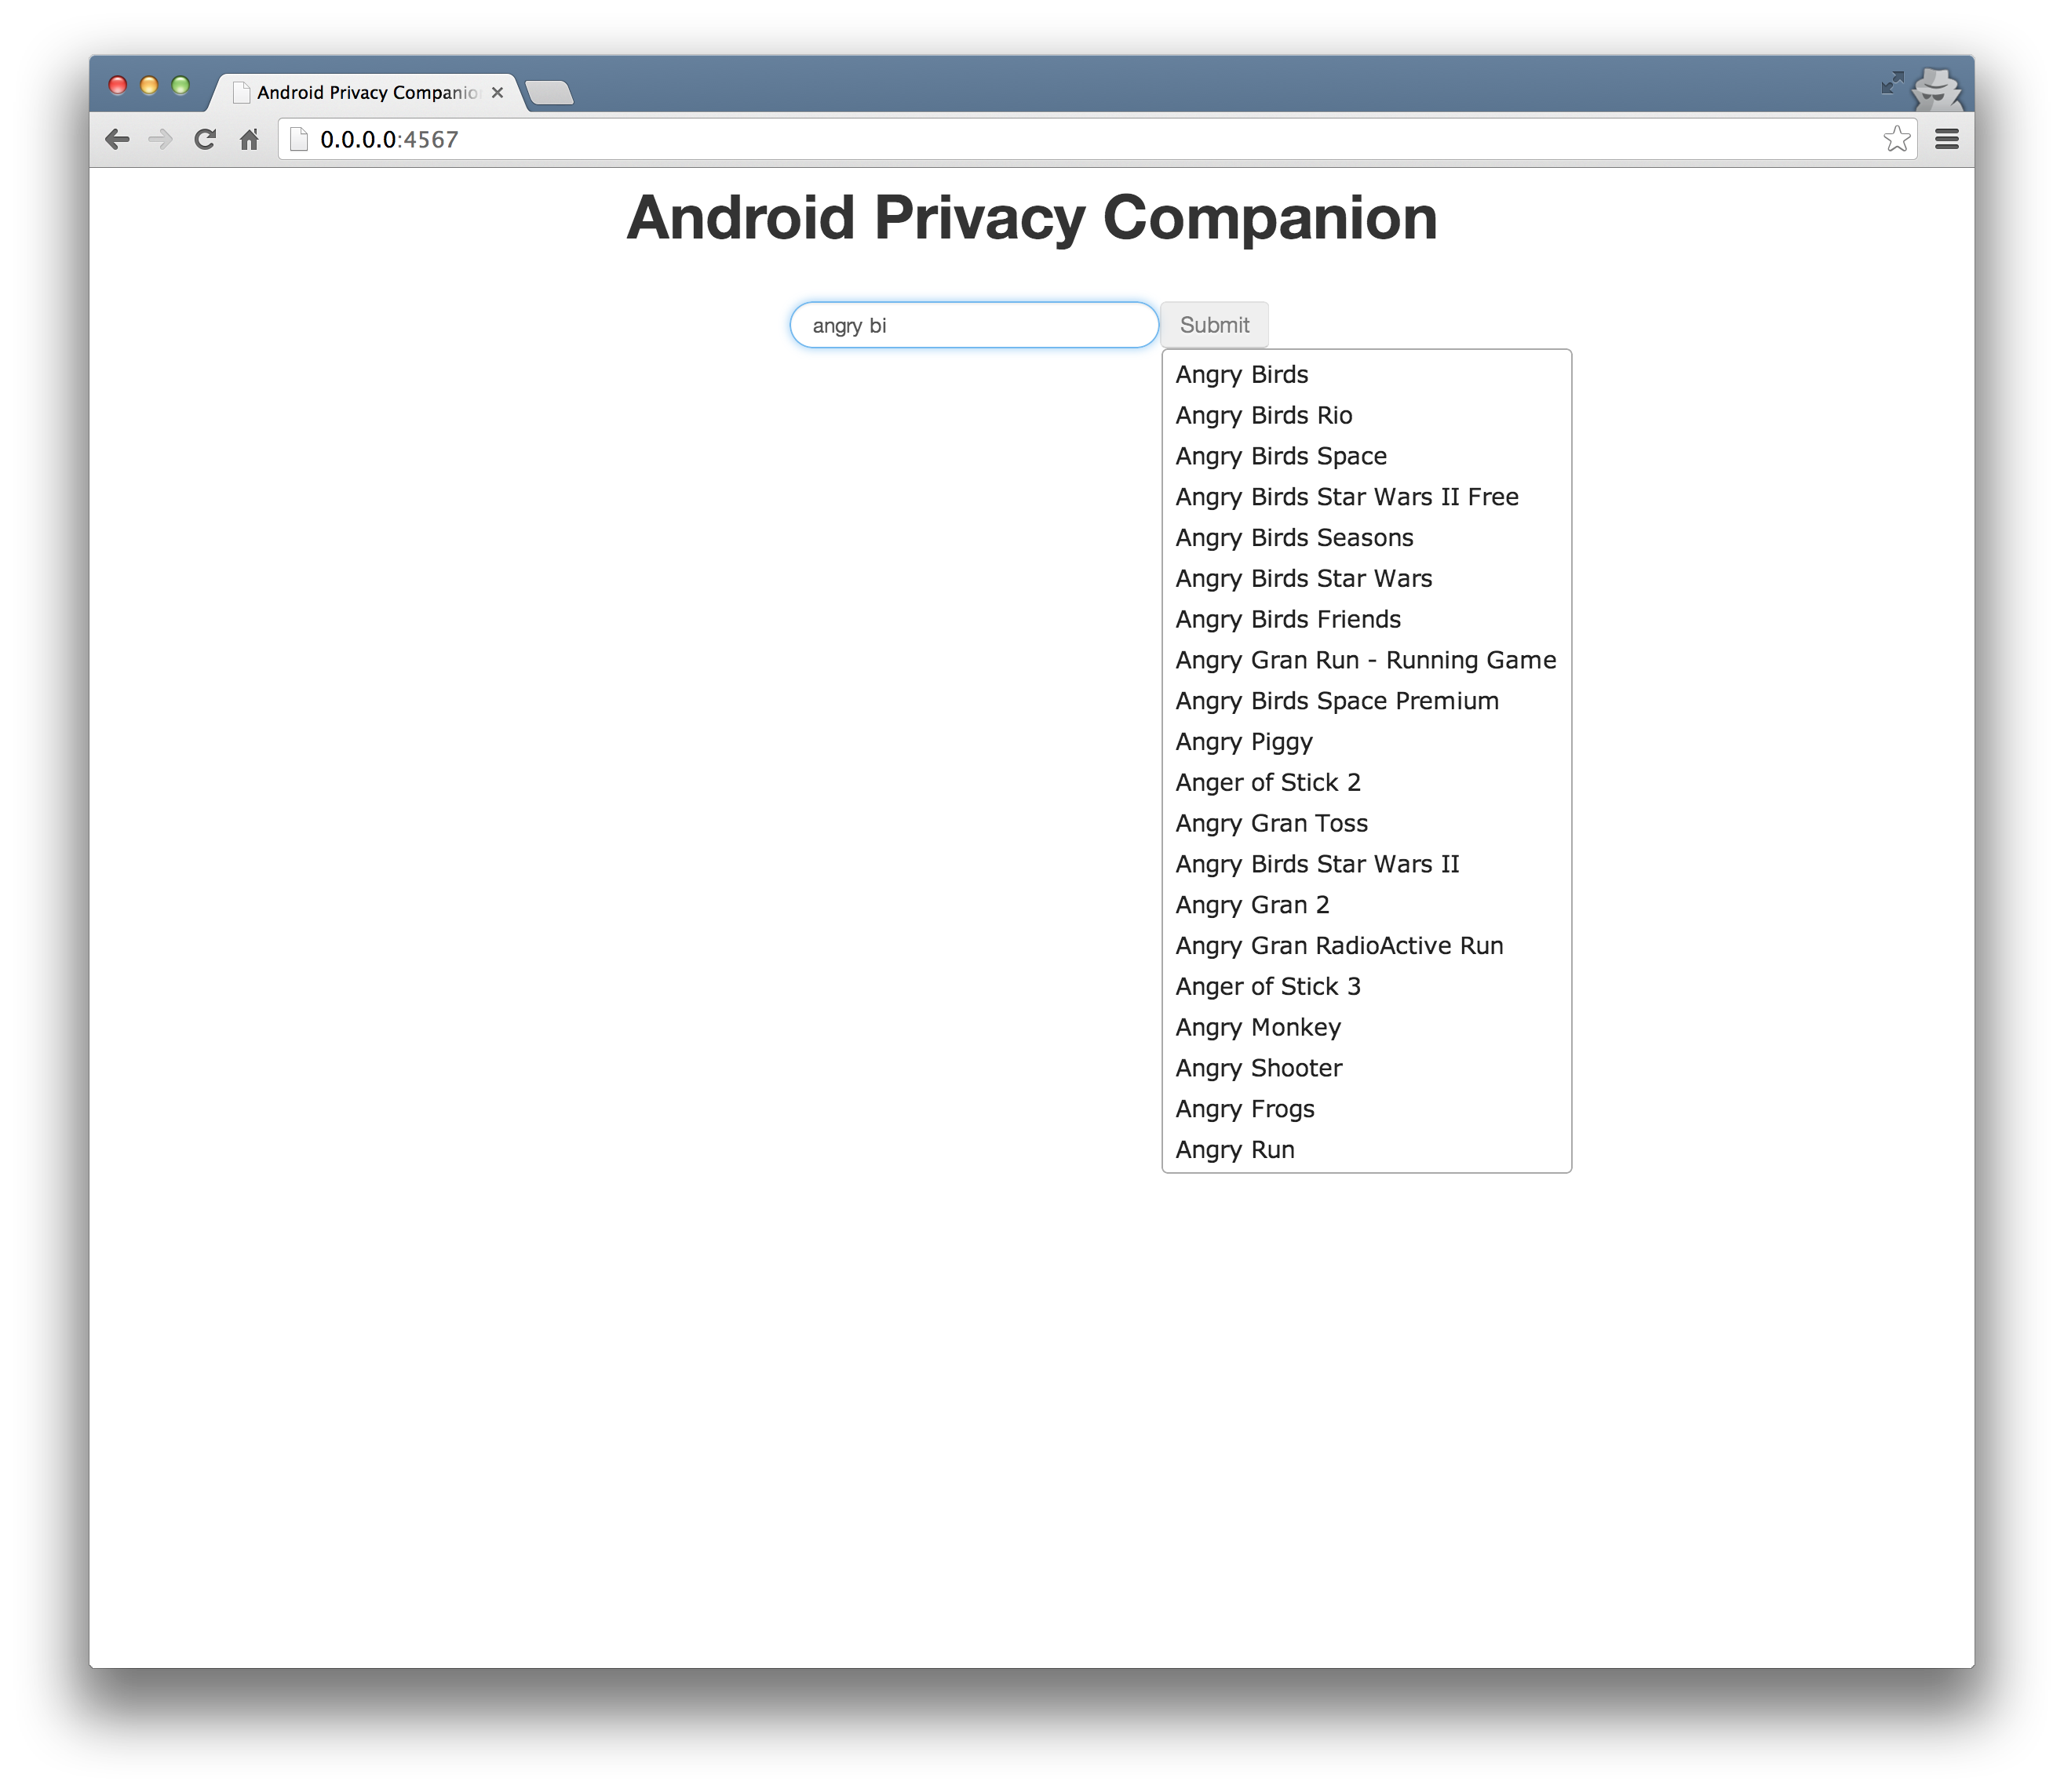
\includegraphics[width=.8\textwidth]{images/example-search}
      \caption{Search interface}
      \label{fig:example-search}
\end{figure}

Once the application has been selected from the list, the permissions list and the privacy policy are automatically retrieved and displayed.
The user can then select one of the permissions requested by the application in order to see all of the relevant sections of the privacy policy.

In \autoref{fig:example-permission-selected} the user selected the \texttt{ACCESS\_COARSE\_LOCATION} permission and a list of relevant sentences is displayed right under the permission description.

\begin{figure}[b]
\centering
     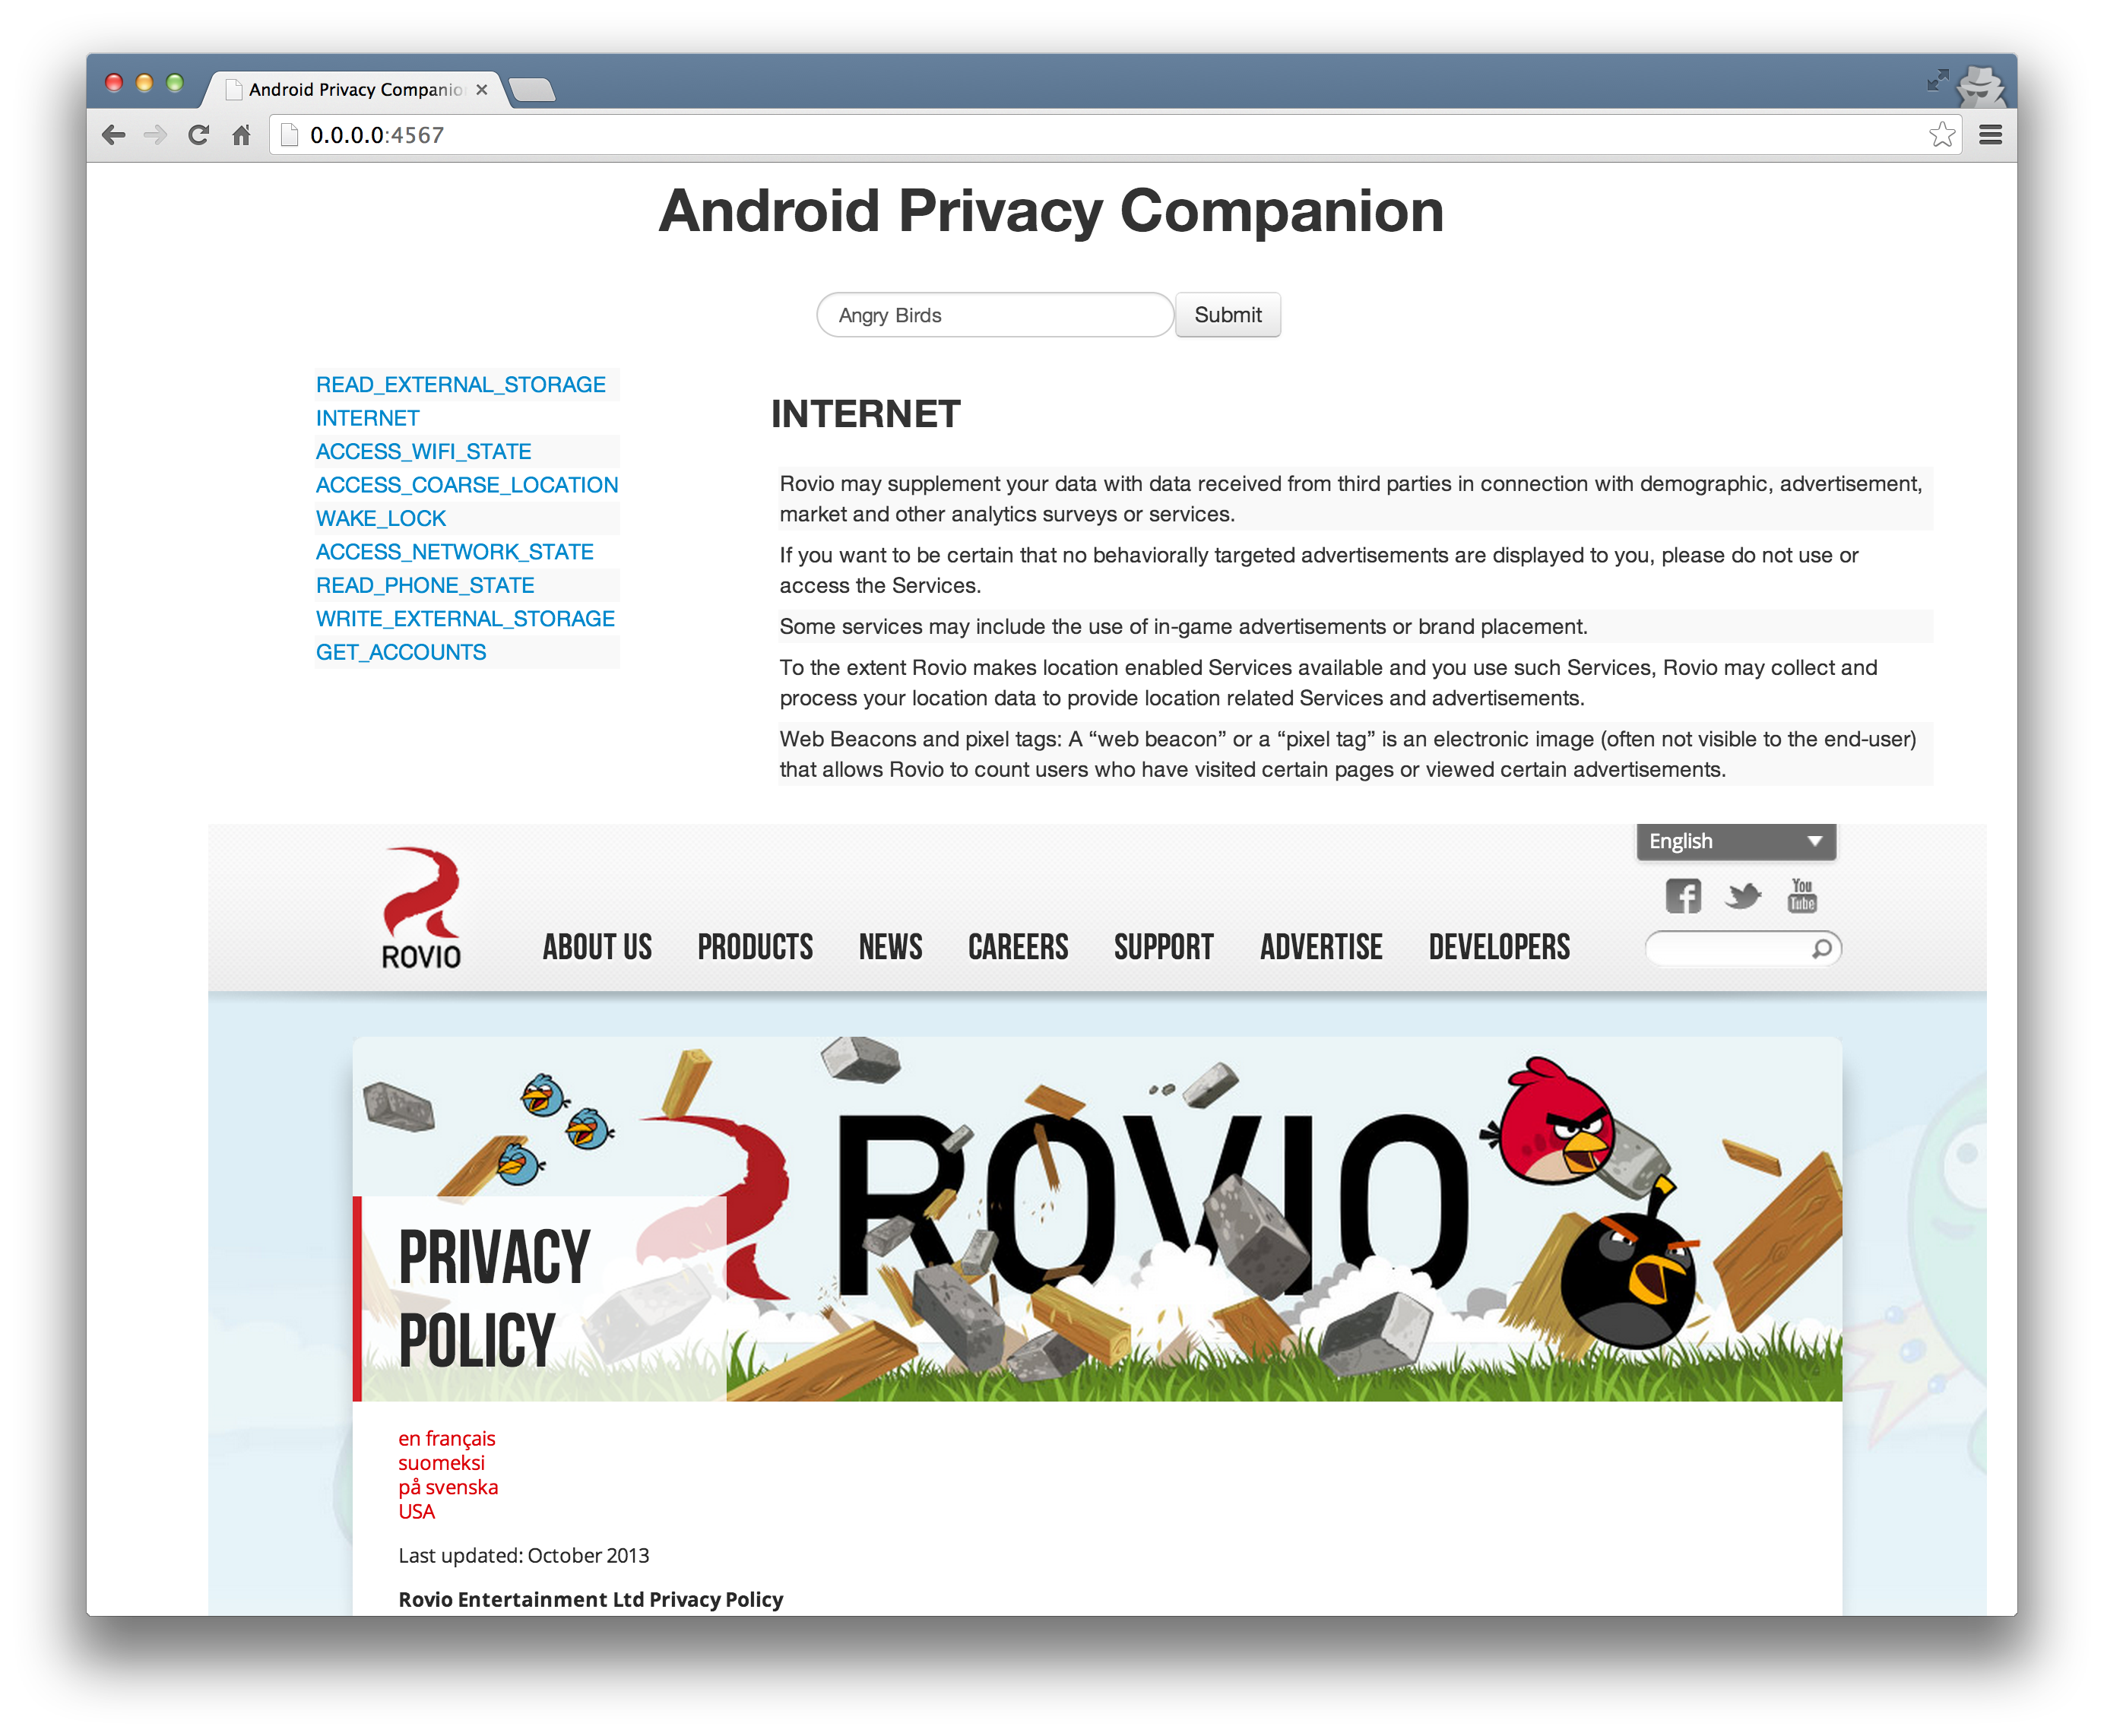
\includegraphics[width=.8\textwidth]{images/example-permission-selected}
      \caption{Permission display interface}
      \label{fig:example-permission-selected}
\end{figure}